\usepackage{graphicx}	% Including figure files
\usepackage{amsmath}	% Advanced maths commands
\usepackage{amssymb}	% Extra maths symbols
\usepackage{multicol}
\usepackage{multirow}
\usepackage{pdflscape}	% Landscape pages
\usepackage{amsmath} % or simply amstext
\newcommand{\angstrom}{\text{\normalfont\AA}}
\usepackage{color}
\usepackage{times}
%\usepackage[space]{grffile}
\usepackage{cleveref}
%\usepackage[normalem]{ulem}
%\usepackage{natbib}
%\usepackage{longtable}
\usepackage{hyperref}
\usepackage{comment}
%\bibpunct{(}{)}{;}{a}{}{,}
\usepackage{url}

This example manuscript is intended to serve as a tutorial and template for
authors to use when writing their own AAS Journal articles. The manuscript
includes a history of \aastex\ and documents the new features in the
previous versions as well as the bug fixes in version 6.31. This
manuscript includes many figure and table examples to illustrate these new
features.  Information on features not explicitly mentioned in the article
can be viewed in the manuscript comments or more extensive online
documentation. Authors are welcome replace the text, tables, figures, and
bibliography with their own and submit the resulting manuscript to the AAS
Journals peer review system.  The first lesson in the tutorial is to remind
authors that the AAS Journals, the Astrophysical Journal (ApJ), the
Astrophysical Journal Letters (ApJL), the Astronomical Journal (AJ), and
the Planetary Science Journal (PSJ) all have a 250 word limit for the 
abstract\footnote{Abstracts for Research Notes of the American Astronomical 
Society (RNAAS) are limited to 150 words}.  If you exceed this length the
Editorial office will ask you to shorten it. This abstract has 182 words.


\begin{figure}
\centering
	% To include a figure from a file named example.*
	% Allowable file formats are eps or ps if compiling using latex
	% or pdf, png, jpg if compiling using pdflatex
	\includegraphics[width=0.8\textwidth]{W1_lc_select.png}
    \caption{WISE light curve in $W1$ band of six CLAGNs with evident long-term infrared variability. }
    \label{fig:W1_lc}
\end{figure}

%%Intrinsic changes in accretion disks are rather a broad concept and may include scenarios with tidal disruption events (i.e SDSS J224113-012108 investigated by Zhang (2021)), tidal interaction between disks in supermassive black hole binaries (Wang & Bon, 2020), the presence and disappearance of the warm corona (Noda & Done, 2018), changes in the magnetization of accretion disk Scepi, Begelman, & Dexter (2021) or magnetic accretion disk-outflows (Feng, Cao, Li,& Gu, 2021).  


from Marzena Śniegowska*1,2 | Mikołaj Grzędzielski2 | Bożena Czerny2 | Agnieszka Janiuk 2021


%2020A&A...643L...9W  Wang Jianmin binary BH
%2020A&A...641A.167S  Czerny disk instability model







\begin{figure}[H]
%\centering
\vspace{-2cm}
\begin{subfigure}
   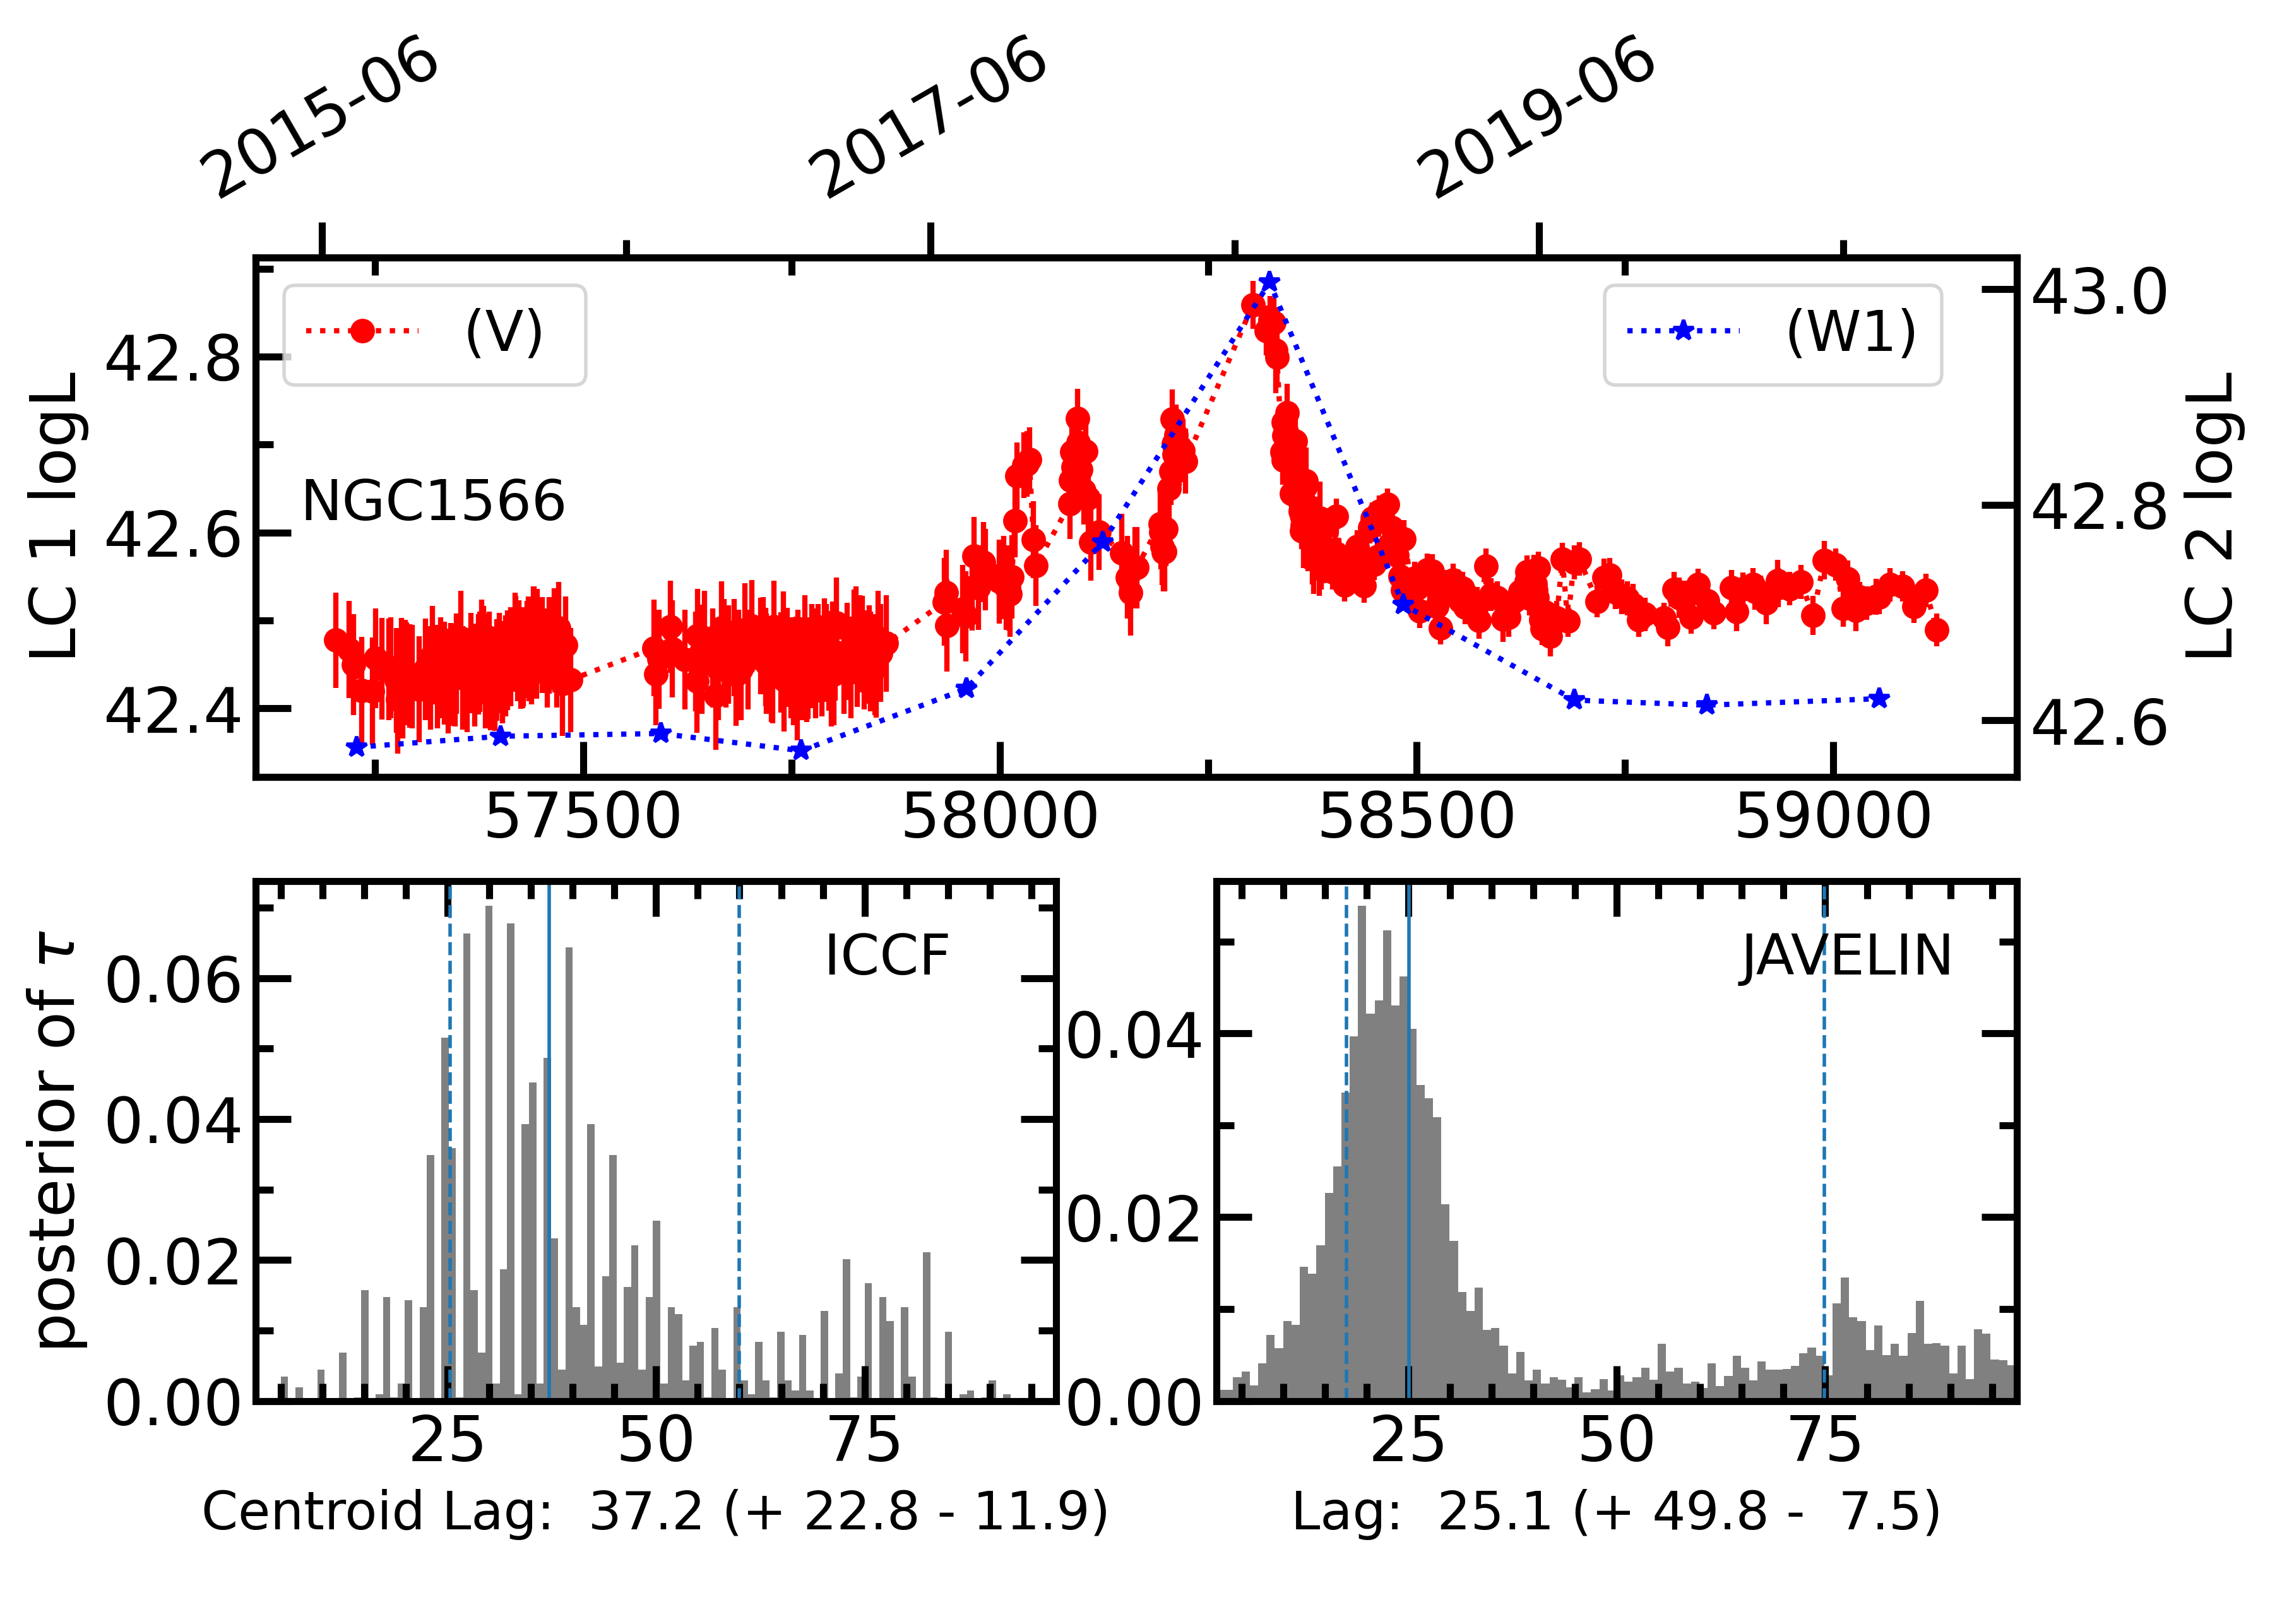
\includegraphics[width=0.45\textwidth]{pic/NGC1566_lag.png}
    %\caption{Dust-reverberation time lag analysis for NGC 1566. }
    \label{fig:lag_NGC1566}
    \end{subfigure}
    \begin{subfigure}
	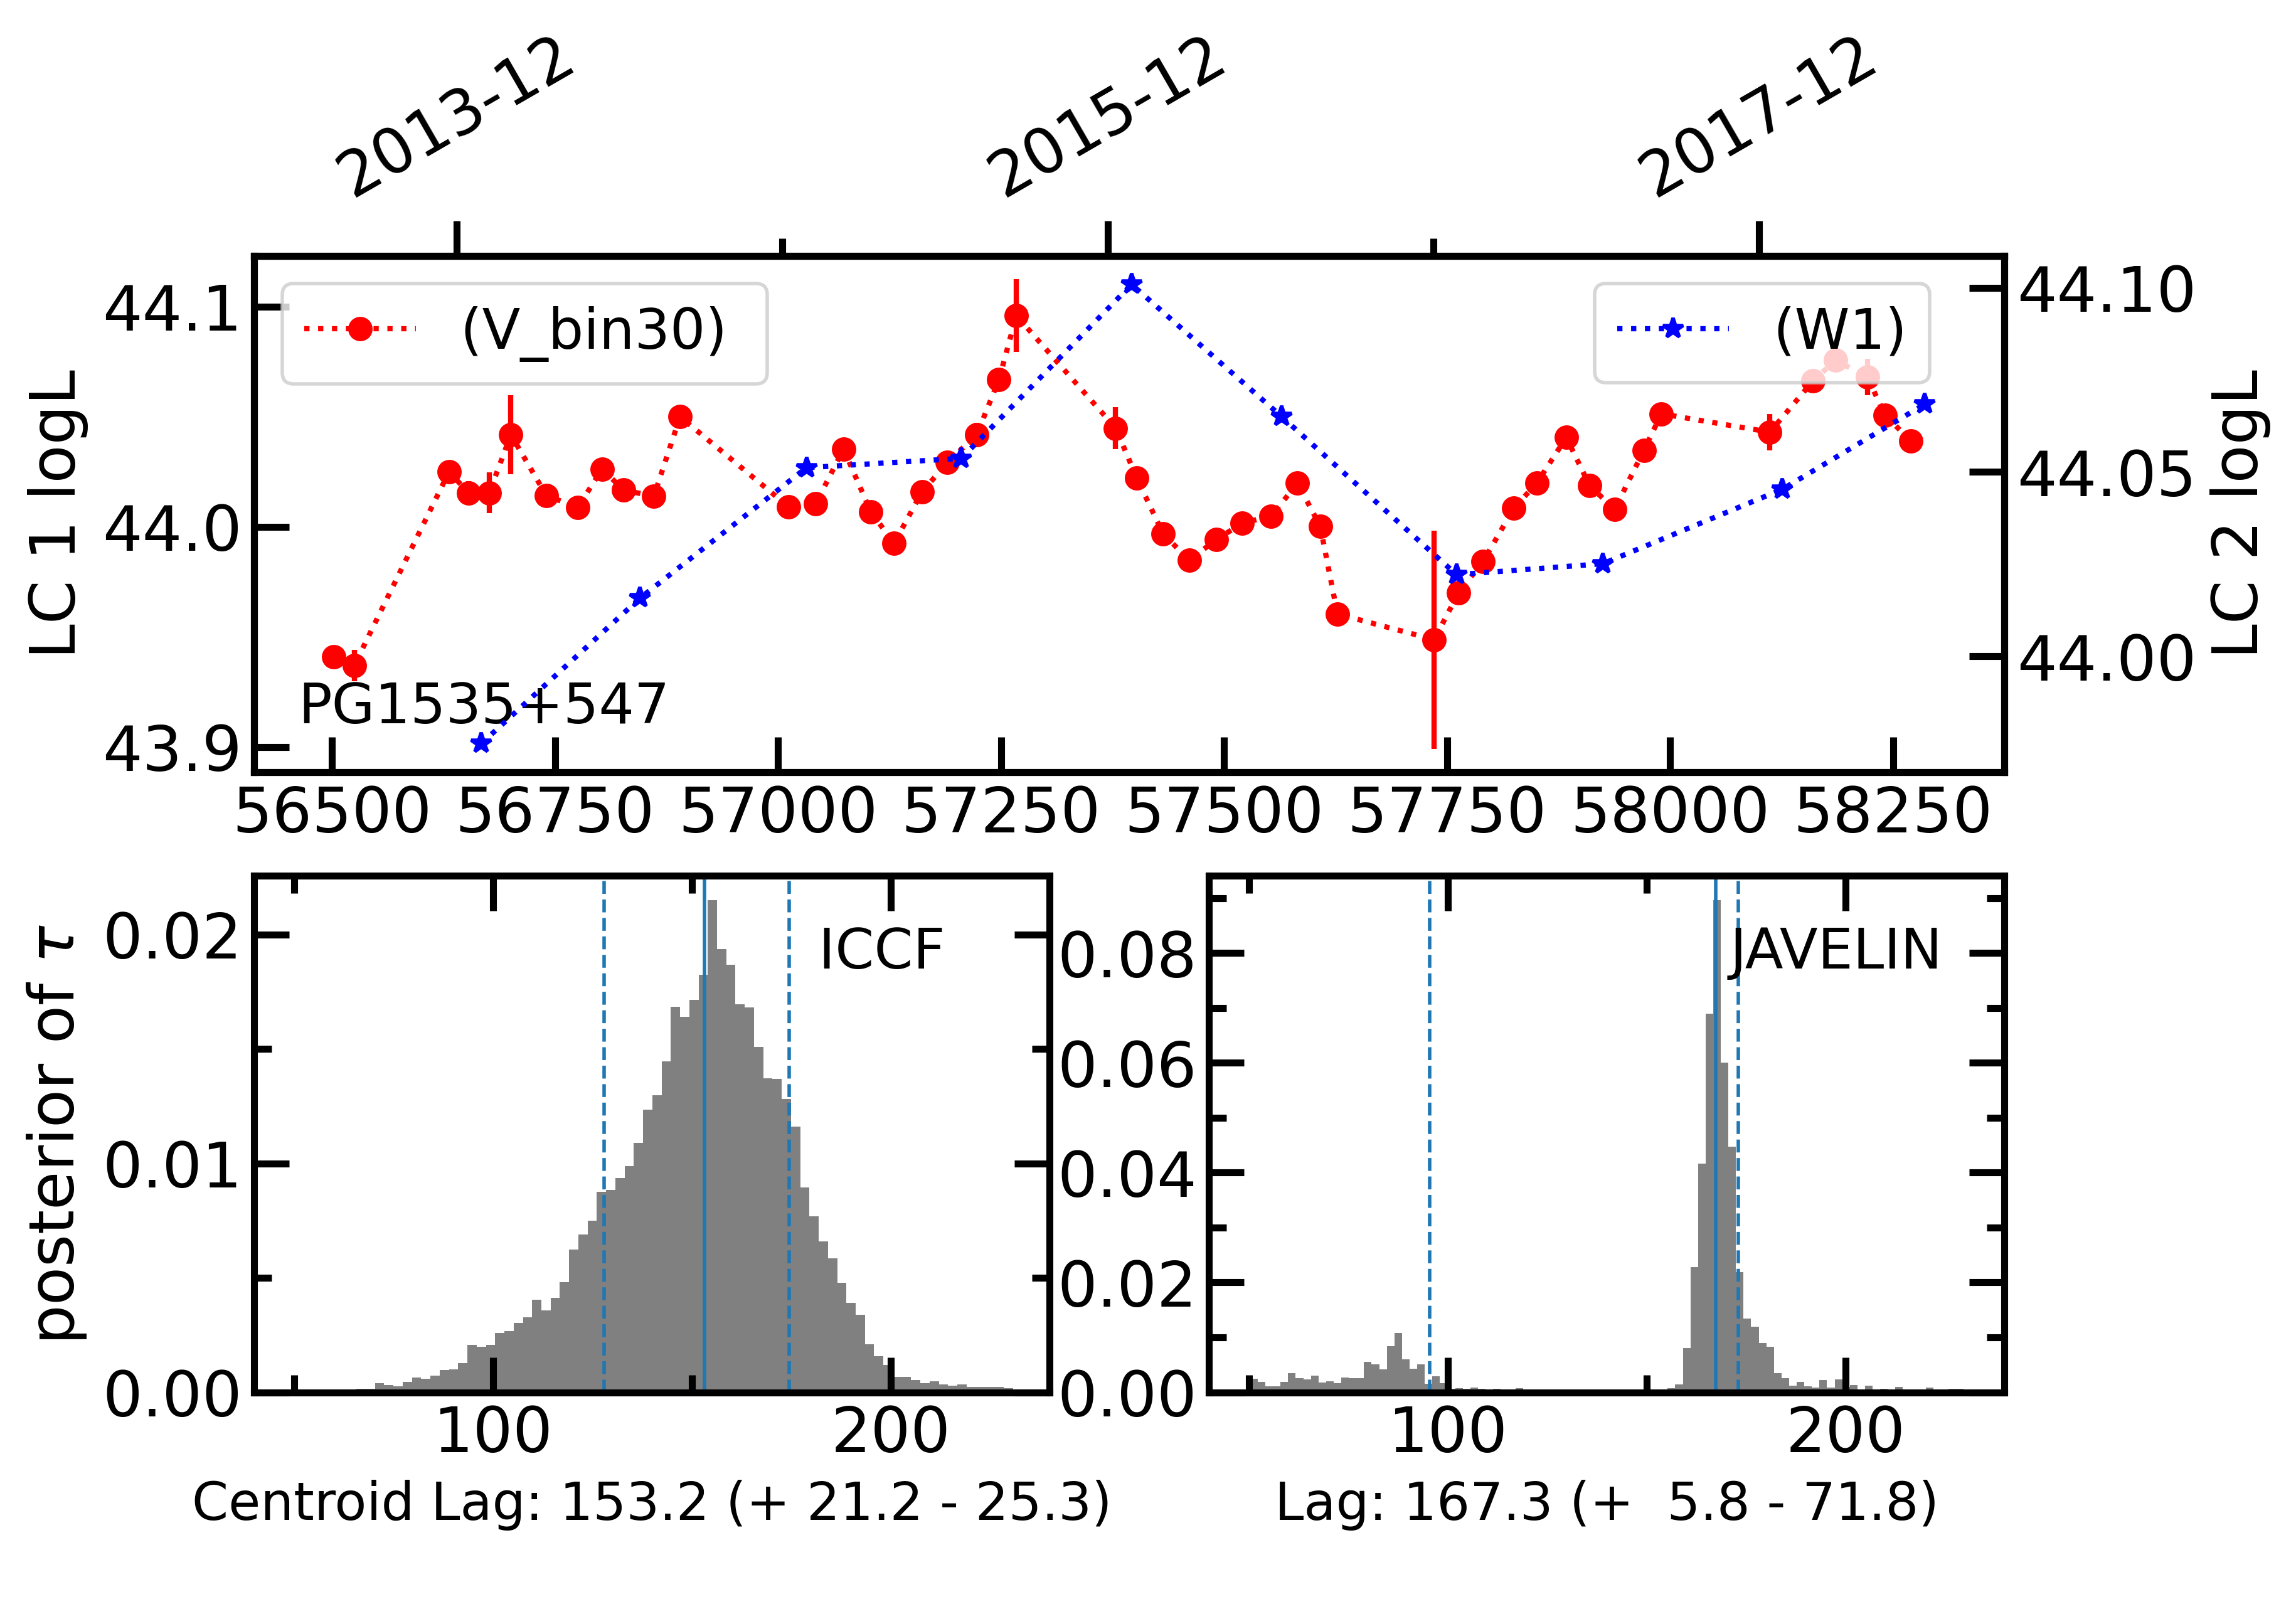
\includegraphics[width=0.45\textwidth]{pic/PG1535p547lag1.png}
    %\caption{Dust-reverberation time lag analysis for PG 1535+547. }
    \label{fig:lag_PG1535}
\end{subfigure}
\end{figure}


\begin{figure}
\begin{tikzpicture}
    \matrix[matrix of nodes]{
    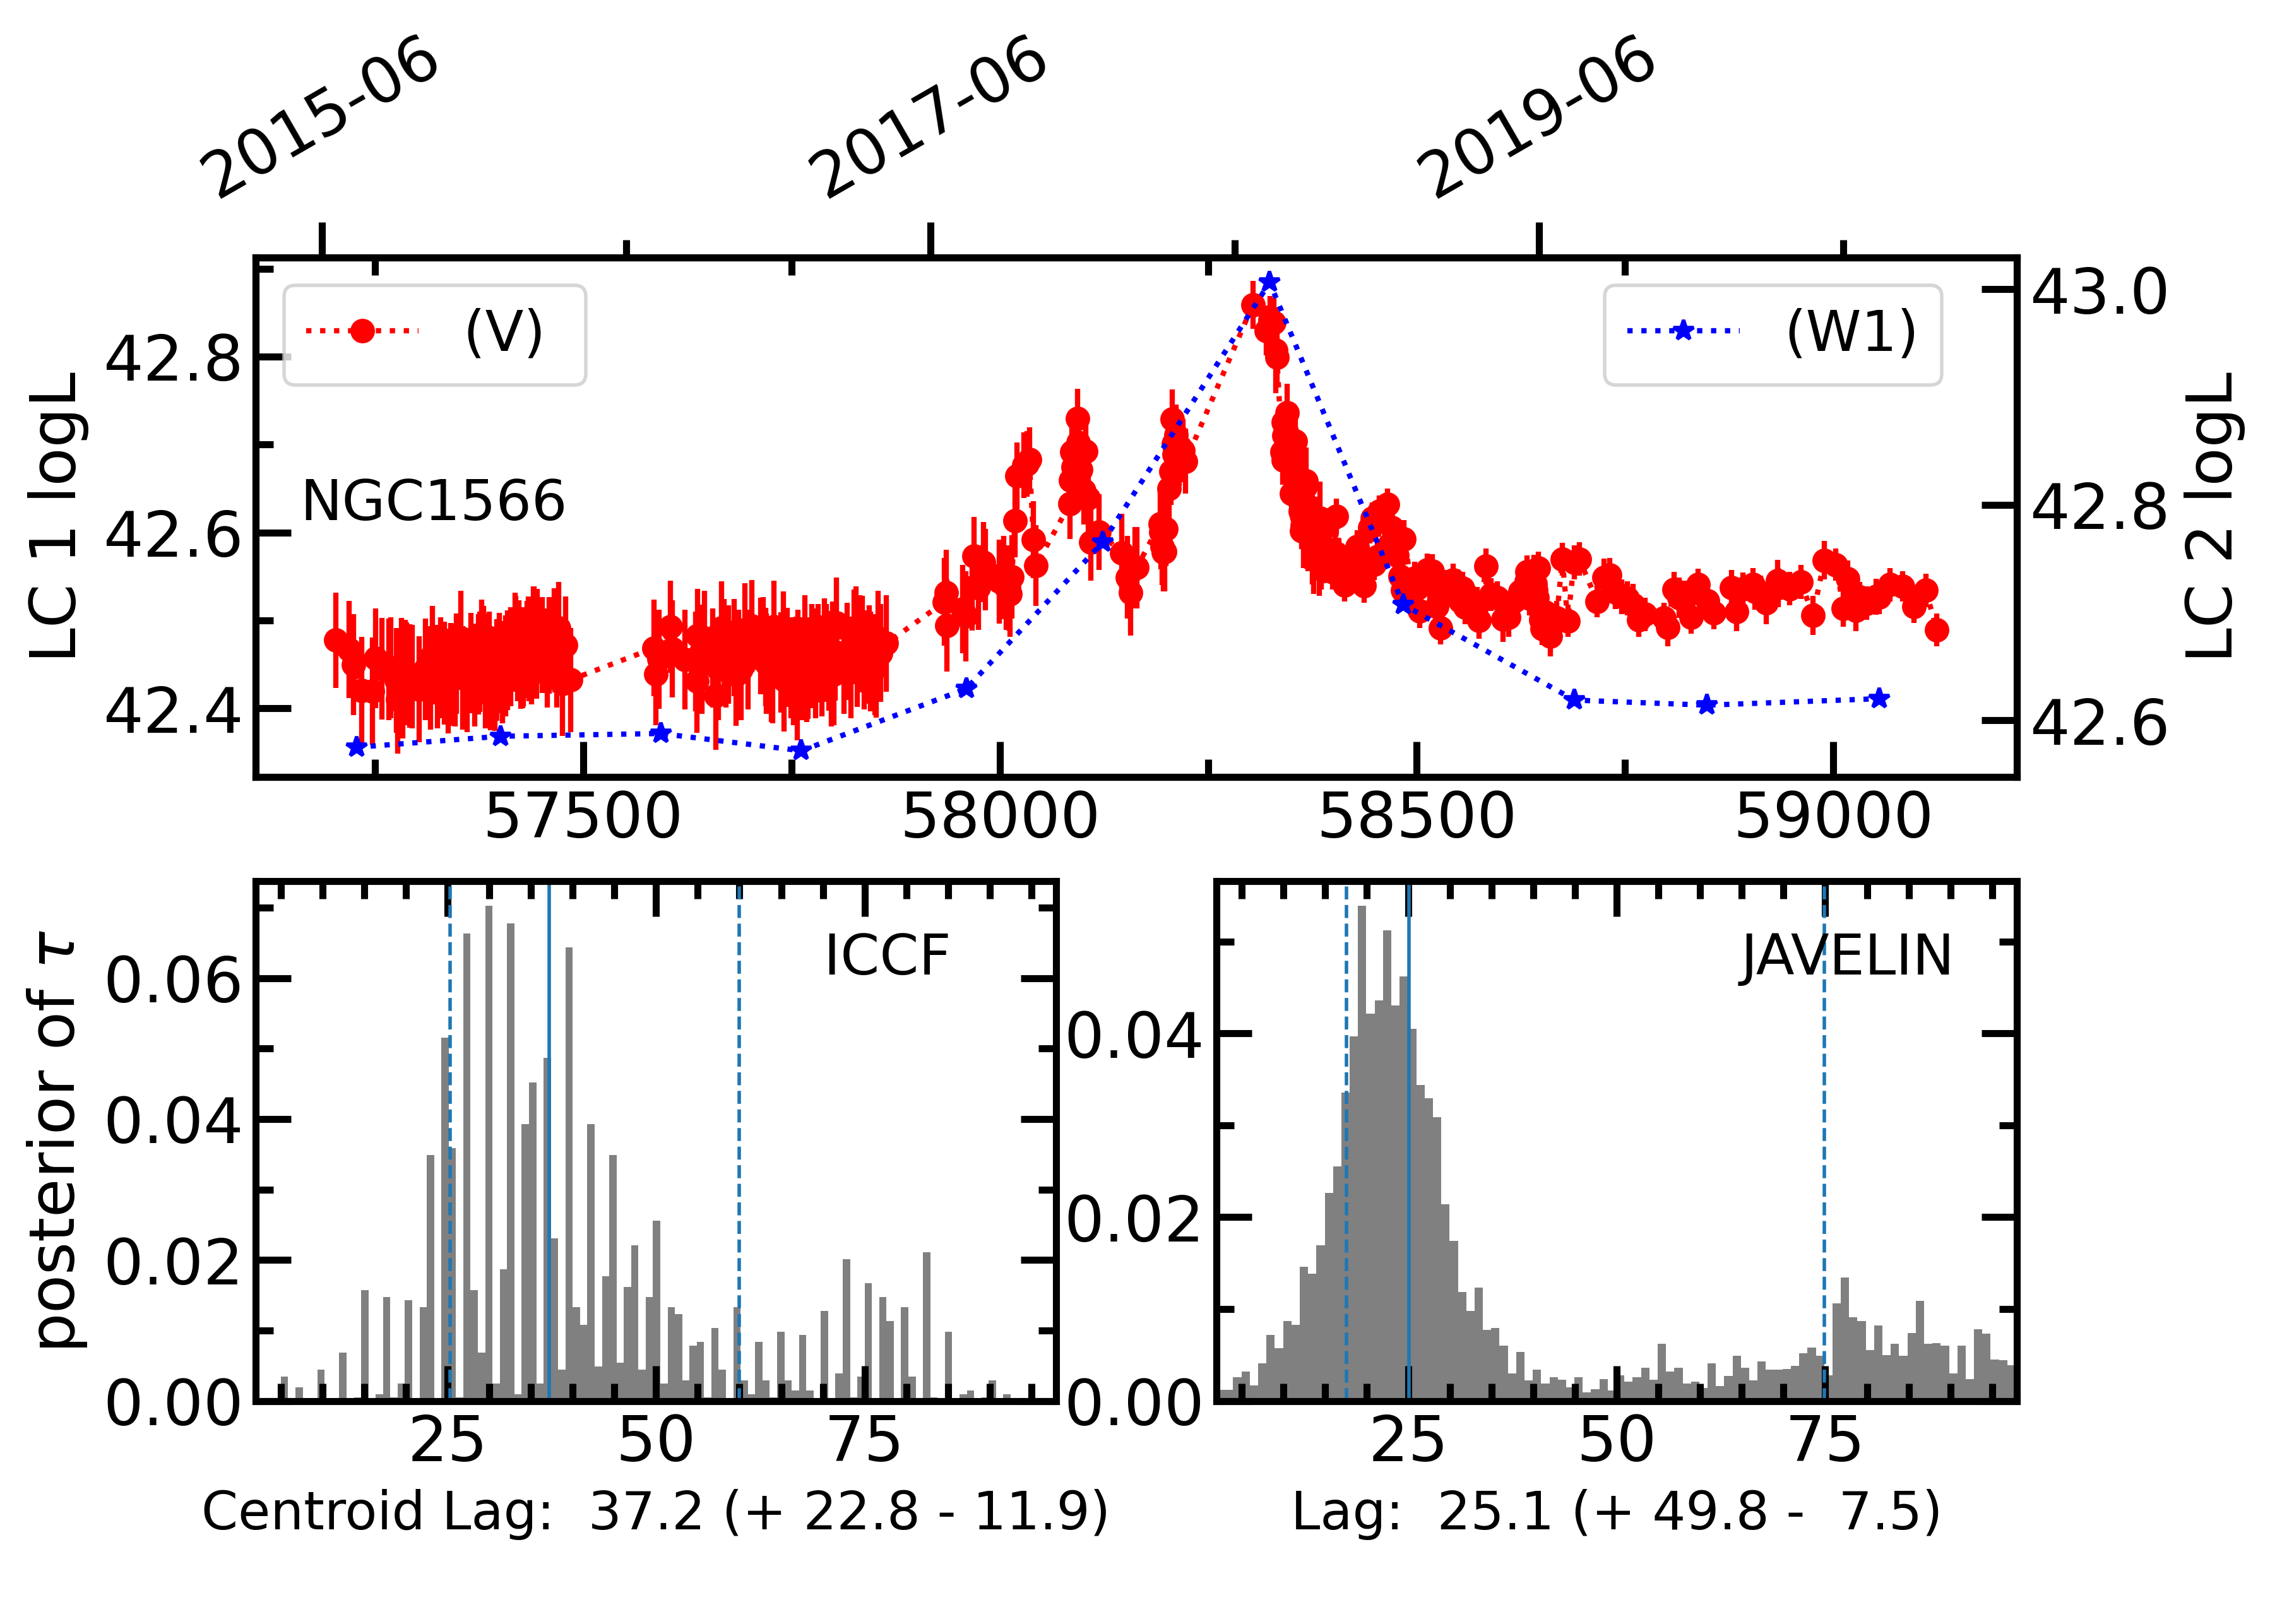
\includegraphics[width=0.45\textwidth]{pic/NGC1566_lag.png}\label{fig:lag_NGC1566} & 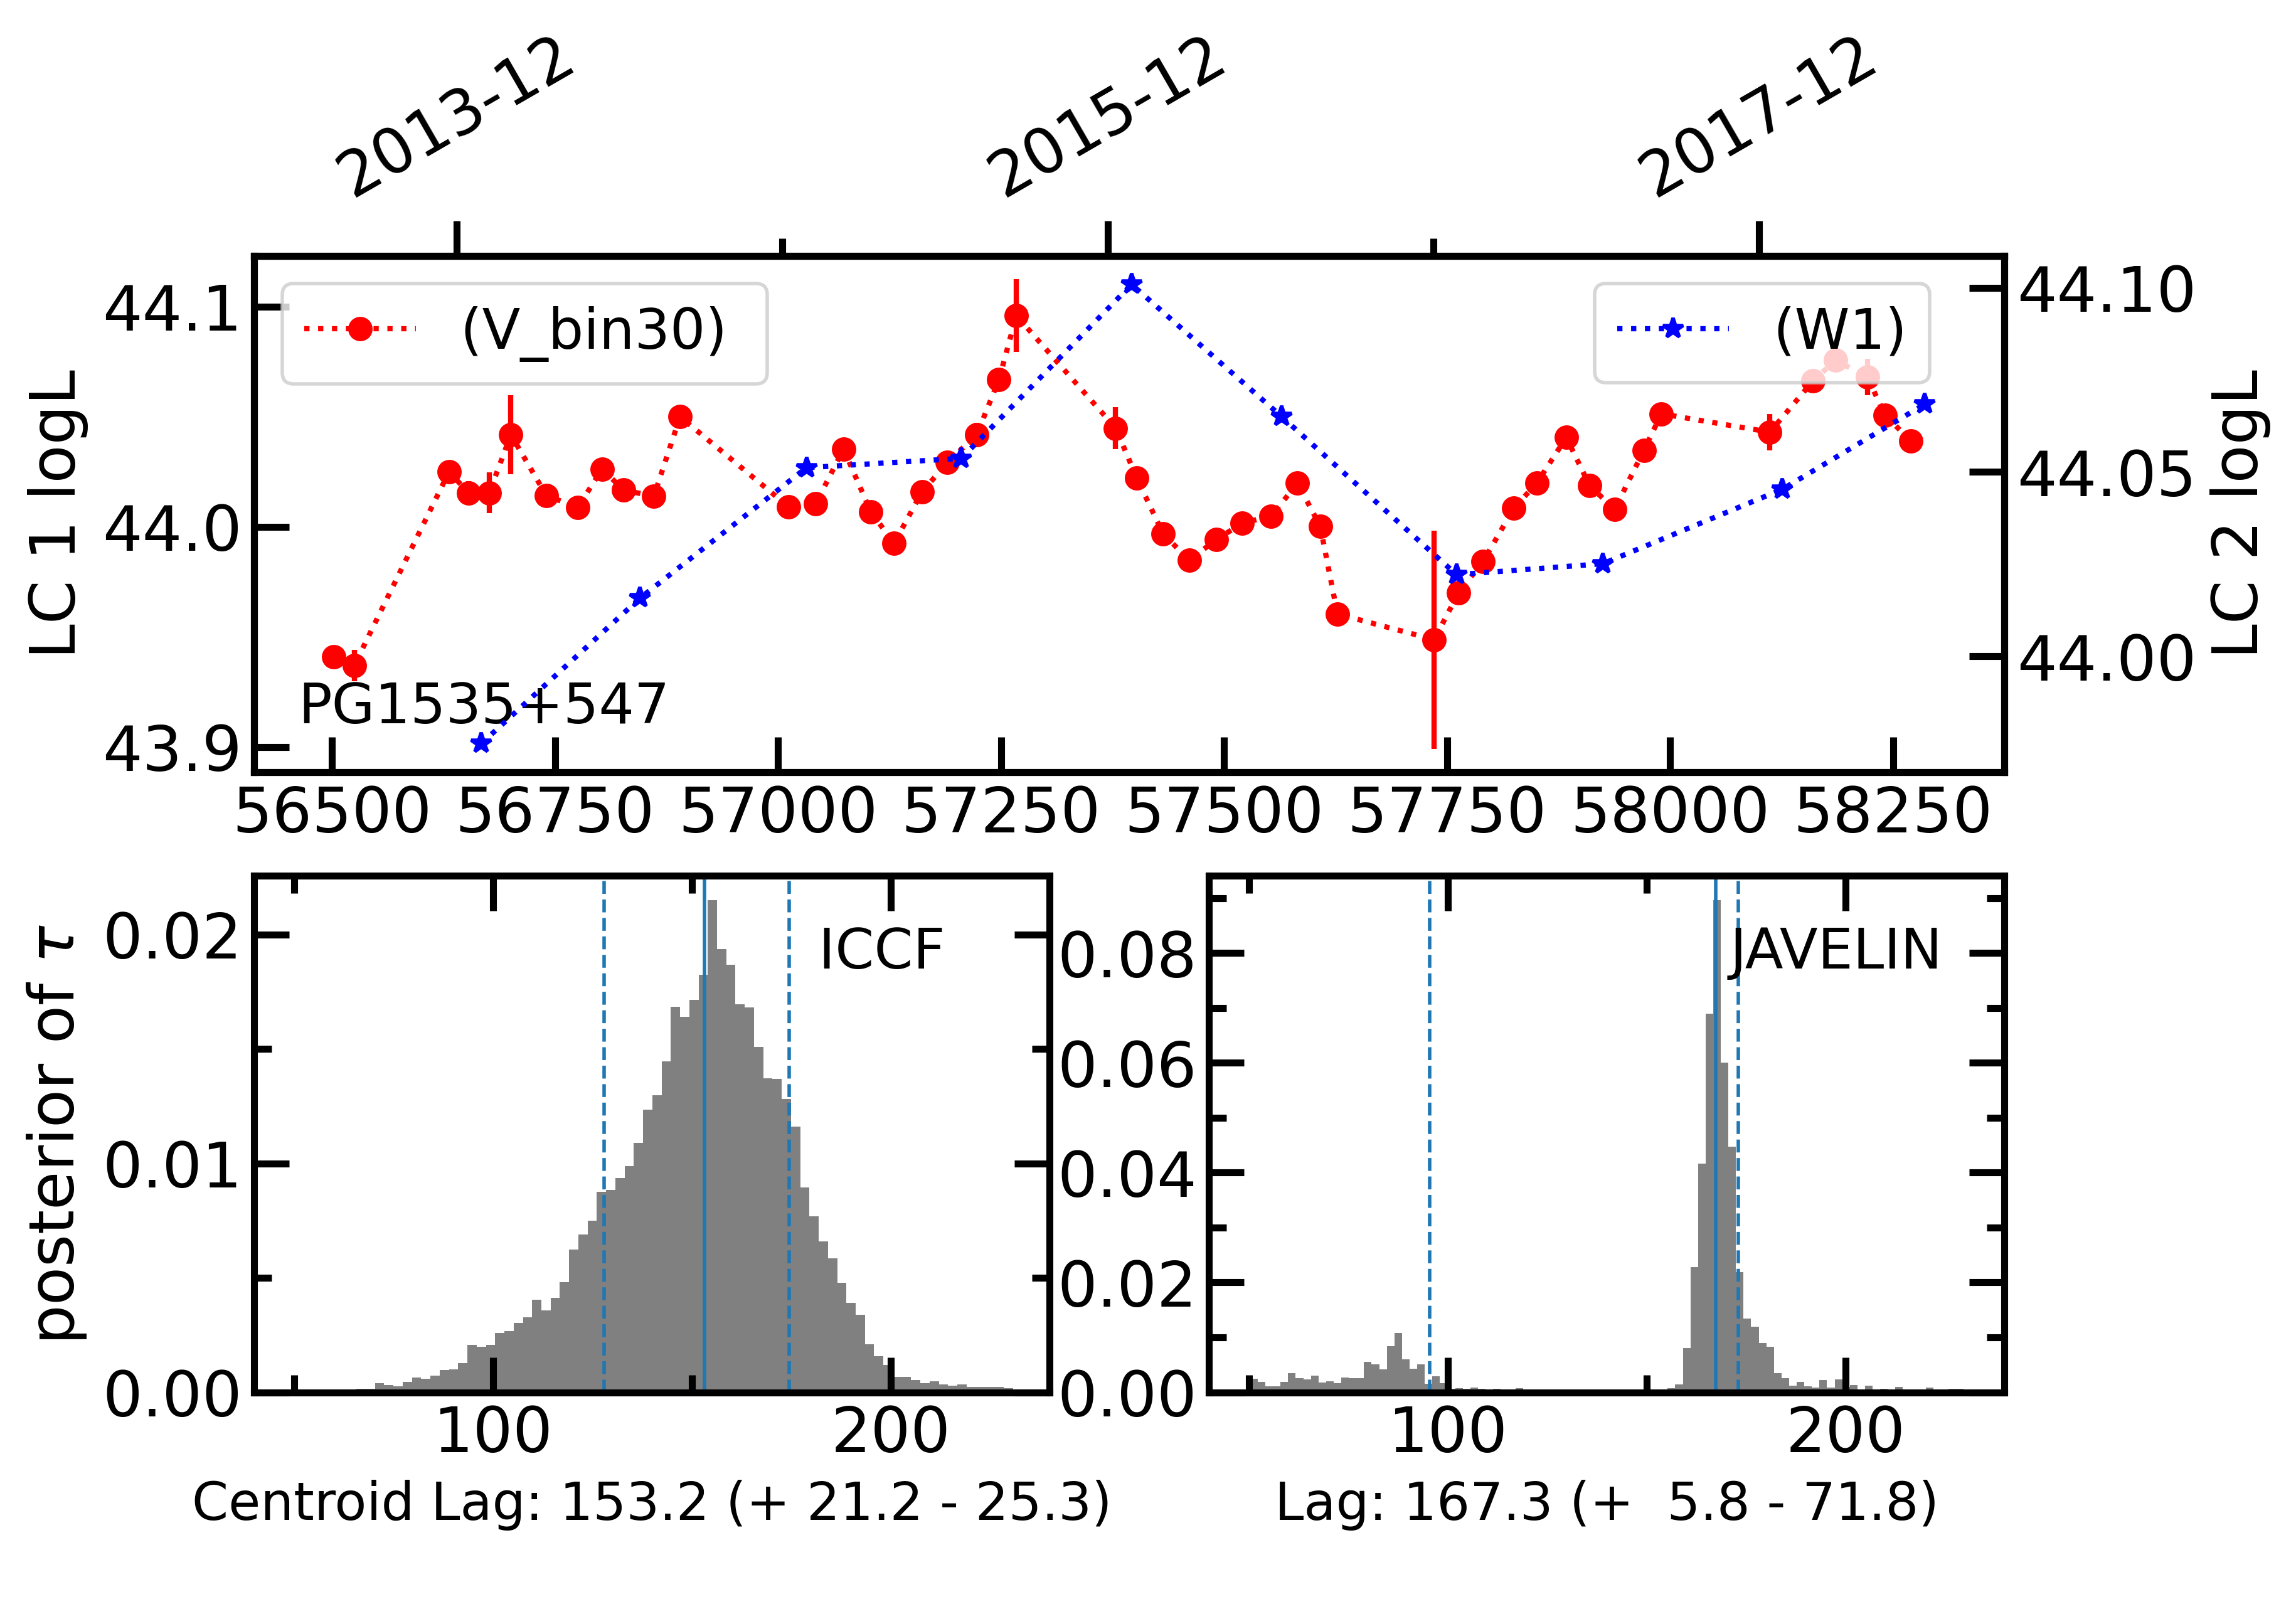
\includegraphics[width=0.45\textwidth]{pic/PG1535p547lag1.png}\label{fig:lag_PG1535} \\
    };
\end{tikzpicture}
\end{figure}


To quantitatively study variability, we calculated the intrinsic 
amplitude of variability ($\sigma_m$), which is the variance of the observed light curve after removing the measurement uncertainty \citep[see also][]{2017ApJ...842...96R}. The $\sigma_m$ is calculated using the following formalism described in \citet{2007AJ....134.2236S}.
\begin{equation}
\Sigma=\sqrt{\frac{1}{n-1}\sum_{i=1}^{N}(m_i - <m>)^2},
\end{equation}
where $m_i$ is the magnitude at $i$-th point and $<m>$ is the weighted average.
The amplitude of variability  can be written as  
$\sigma_m$ is             
\[\sigma_m  =
  \begin{cases}
    \sqrt{\Sigma^2 - \epsilon^2},  & \quad \text{if } \Sigma>\epsilon,\\
     0,                            & \quad  \text{otherwise.}\\
  \end{cases}
\]	               
where the error $\epsilon$ is calculated from the individual errors as follows
\begin{equation}
\epsilon^2=\frac{1}{N}\sum_{i=i}^{N}{\epsilon_{i}^{2} + \epsilon_{s}^2}. 
\end{equation}
Here $\epsilon_{i}$ is the measurement uncertainty of $i$-th point and $\epsilon_{s}$ is the systematic uncertainty. \citet{2011ApJ...735..112J} reported systematic uncertainties of 0.024 mag and 0.028 mag in $W$1 and $W$2 respectively. Therefore, this error has been added in quadrature to the measurement uncertainty and thus taking care of systematic as well as random errors. Spurious correlation may occur if $\sigma_m$ is not corrected for the redshift of the object, especially important for a flux-limited sample, we, therefore, calculated rest frame $\sigma_m$ by multiplying $\sigma_m$ with $\sqrt{(1+z)}$, which is based on the power spectral
density of variability having slope 2 \citep[see][]{2009ApJ...698..895K}. However, the majority ($\sim 87\%$) of the variable candidates in our sample is below $z=0.4$, thus, redshift correction is insignificant.















\subsection{X-ray data}
\subsubsection{\xrt}
The X-ray telescope (XRT) onboard \swift\, has high cadence-monitoring observations of the CLAGN sample. We use {\sc xselect} to extract the source and background spectra. The spectra are grouped by the a minimum of one count per bin. The XRT spectra in the 0.5--10~keV range are fitted by an absorbed power-law model \texttt{tbabs*zpowerlw} with the Galactic hydrogen absorption using the Bayesian X-ray Analysis software BXA \footnote{\url{http://johannesbuchner.github.io/BXA/index.html}} \citep[][]{2014A&A...564A.125B}.


\subsubsection{\maxi}
\textit{MAXI} \citep{2009PASJ...61..999M} onboard the International Space Station (ISS) performed all-sky monitor since 2009 August 15 with the Gas Slit Cameras (GSCs; \citealt{2011PASJ...63S.623M}) 
  in 2--30~keV and the Solid-state Slit Cameras (SSC; \citealt{2011PASJ...63..397T}) in 0.5--12~keV. Several CLAGNs has been monitored almost daily by \textit{MAXI}.  We extracted the light curves of CLAGNs with 1 day bin \footnote{\url{http://maxi.riken.jp/top/slist.html}}. 

  


\subsection{Optical V-band data}
\subsubsection{\uvot\,V-band}
 We use the tool \textit{uvotsource} to do the aperture photometry for V-band data of \uvot\,. The source aperture radius is 5$\arcsec$ and the background is chosen in a blank region with a much larger radius.


\subsubsection{ASAS-SN\,V-band data}
We used the photometric data of NGC 1566 from the ASAS-SN \citep[All-sky Automated Survey for Supernovae,][]{2014ApJ...788...48S,2017PASP..129j4502K,2019MNRAS.485..961J}. ASAS-SN \citep[][]{2018ATel11893....1D} reported the brightening of NGC 1566 around September 2017, which is brightest in July 2018. We determined the average offset between the simultaneous (within 1 day of interval) ASAS-SN and \uvot\, V-band data. Then the ASAS-SN\,V-band magnitude was reduced to the V-band of \uvot\, system.



\begin{figure}
\centering
	% To include a figure from a file named example.*
	% Allowable file formats are eps or ps if compiling using latex
	% or pdf, png, jpg if compiling using pdflatex
	\includegraphics[width=0.9\textwidth]{pic/wisename_varO_0.2.png}
    \caption{{\it WISE} light curves of Optical selected CLAGNs with $\sigma_{m W1} > 0.2$. }
    \label{fig:O-CLAGN-lc}
\end{figure}


\begin{figure}
\centering
	% To include a figure from a file named example.*
	% Allowable file formats are eps or ps if compiling using latex
	% or pdf, png, jpg if compiling using pdflatex
	\includegraphics[width=0.5\textwidth]{pic/wisename_varO_left.png}
    \caption{{\it WISE} light curves of Optical selected highly variable CLAGNs for illustration.} 
    \label{fig:O-CLAGN-lc-left}
\end{figure}


\begin{figure}
\centering
	% To include a figure from a file named example.*
	% Allowable file formats are eps or ps if compiling using latex
	% or pdf, png, jpg if compiling using pdflatex
	\includegraphics[width=0.8\textwidth]{pic/wisename_varO_mag0.4.png}
    \caption{{\it WISE} light curves of Optical selected highly variable CLAGNs for illustration. The black dashed line marks the epoch when the source is Type 1. The black dot-dashed line marks the epoch when the source is Type 1.5. The grey dotted line marks the epoch when the source is Type 1.9/2.} 
    \label{fig:O-CLAGN-lc}
\end{figure}


\subsection{MIR variability timescale}
We fited the light curves using a damped random walk model in {\sc javelin} algorithm \citep[][]{2011ApJ...735...80Z,2013ApJ...765..106Z} to estimate the MIR variability timescale. We limited the range of timescale within $90-10^{6}$ days due to its 180 day's sampling rate and 10 year's monitoring. We find the distributions of timescale are guassian-like with log${\uptau _{W1}}\sim 2.35\pm 0.01$ and log ${\uptau_{W2}}\sim 2.47\pm 0.02$. The ratio between ${\uptau _{W1}}$ and ${\uptau _{W2}}$ is $\sim 3:4$ ($225:298$). We ploted the distributions of MIR variability timescale in \autoref{fig:distribution_MIRtimescale}.

\begin{figure}
\centering
	% To include a figure from a file named example.*
	% Allowable file formats are eps or ps if compiling using latex
	% or pdf, png, jpg if compiling using pdflatex
	\includegraphics[width=0.45\textwidth]{pic/WISE_timescale.png}
    \caption{Distribution of the MIR variability timescale ($\uptau$) of CLAGNs.}
    \label{fig:distribution_MIRtimescale}
\end{figure}


%2017PASP..129j4502K
%At the resolution of ASAS-SN, the local crowding will tend to change the light curve by some constant in flux, distorting its shape
% Contamination due to the local crowding will generally distort an ASAS-SN light curve by an additive constant in flux.


Combining the results from literature, we plot the dust-reverberation time lag ($\tau_{W1}$) and bolometric luminosity ($L_\mathrm{bol}$) relation of AGNs in \autoref{fig:tau_L}. \citet[][]{2019ApJ...886...33L} reported that the inferred dust emission size ratios $R_\mathrm{K}$: $R_{W1}$: $R_{W2}$ are $0.6: 1: 1.2$. So we multiplied $\tau_\mathrm{K}$ in \citet[][]{2014ApJ...788..159K,2019ApJ...886...33L} by a factor of 5/3. We used UltraNest\footnote{\url{https://johannesbuchner.github.io/UltraNest/}} package \citep{2021JOSS....6.3001B} to fit the linear log$\tau$-log$L_{bol}$ relation for Type 1s, Type 2s, and CLAGNs with errors considered. The fitting results show a slope of $0.36 \pm 0.04$, an offset of $2.13 \pm 0.03$, and a scatter of $0.17 \pm 0.02$. Though the slope ($0.36 \pm 0.04$) is slightly lower than the slope ($0.47 \pm 0.06$) from fitting of PG quasars in \citet[][]{2019ApJ...886...33L}, the $\tau$-$L_{bol}$ relation are consistent for CLAGNs and normal AGNs with scatter.


%Seyfert 1.5 galaxy Mrk 530 experienced twice ``changing-look'' \citep{2019sf2a.conf..509M} during 1974-1998 and underwent a transition from a soft to hard spectrum with \suzaku\, in 2012 \citep{2018MNRAS.478.4214E}. The MIR light curve shows gradually decline of luminosity in recent years.


%NGC 7582 is a X-ray bright Seyfert galaxy, which changed from type 2 to type 1 in 1998 \citep{2019sf2a.conf..509M}. NGC 7582 showed highly variable absorption features around 2000 \citep{2015ApJ...815...55R}. NGC 7582 experienced an outburst in MIR band around November 2018, reached the bright luminosity level around November 2010. NGC 7582 are slowly dimming.

%\subsection{MIR Variability timescale}


%\subsection{Possible mechanism for ``changing-look'' }
%NGC 1566, NGC 4151 and NGC 5548 experienced multiple outbursts \citep{2020A&A...641A.167S}. 
%The long-term MIR variability of some sources (e.g. NGC 4051, NGC 4151, NGC 4395, NGC 5548) is also complex. 


%\subsection{Sources might be changing look again?}








%\section{Discussion} \label{sec:dis}

Different wavelength emissions come from the different regions of AGN. 

%can well explain the multi-wavelength observations of different AGNs with high- (quasars), intermediate- (e.g. Seyferts), and low-nuclear luminosity (LLAGNs).

%Besides, the disk-wind might influence the X-ray spectrum with the evolution of accretion disk.


%The MIR luminosity variability of both Optical and X-ray selected CLAGNs directly response to the transitional accretion process according to the $\tau$-$L_\mathrm{bol}$ correlation. 

%The nagative/positive X-ray photon index and optical/UV to X-ray spetral index$\alpha_\mathrm{OX}$ with luminosity correlation below/above a critical luminosity $L_\mathrm{AGN}/L_\mathrm{Edd} \sim 0.01$ support different accretion mode in different luminosity for a sample of X-ray Binaries and AGNs \citep[e.g.][]{2015MNRAS.447.1692Y,2011ApJ...739...64X,2017MNRAS.471.2848L}. 

%\simga_m$
%in both optical and X-ray selected changing-look AGNs

\citet{2014ARA&A..52..589H} separates AGNs into two major groups: radiative-mode AGNs and jet-mode AGNs. 

The re-scaled $\tau_{W1} \sim 146 $  days of NGC 7469 in \citet[][]{2014ApJ...788..159K} is consistent with $\tau_{W1}$ $\sim 131.2^{+37.9}_{-22.4}$ days of NGC 7469 in this work.


Mrk 590 & 43.84 & $ 33.8 \pm 4.20$ & O & \citet{2014ApJ...788..159K} \\
NGC 3516 & 43.62 & $ 73.1 \pm 4.00$ & O & \citet{2014ApJ...788..159K} \\
NGC 4051 & 42.66 & $ 16.5 \pm 0.60$ & X & \citet{2014ApJ...788..159K} \\
NGC 4151 & 43.62 & $ 48.3 \pm 0.50$ & O & \citet{2014ApJ...788..159K} \\
NGC 5548 & 43.87 & $ 60.9 \pm 0.30$ & O & \citet{2014ApJ...788..159K} \\
NGC 7469 & 44.28 & $ 88.0 \pm 0.60$ & X & \citet{2014ApJ...788..159K} \\
NGC 3516 & 43.84 & 53.6 & O & \citet{2019ApJ...886...33L} \\
NGC 4051 & 42.88 & 12.9 & X & \citet{2019ApJ...886...33L} \\
NGC 4151 & 43.84 & 52.2 & O & \citet{2019ApJ...886...33L} \\
NGC 5548 & 44.07 & 50.5 & O & \citet{2019ApJ...886...33L} \\
NGC 7469 & 44.45 & 56.1 & X & \citet{2019ApJ...886...33L} \\


The time lag results from \citet{2014ApJ...788..159K} and \citet{2019ApJ...886...33L} are between V band and K band.%, which are scaled to $\tau_\mathrm{W1}$ with $\tau_\mathrm{W1}=\tau_\mathrm{K} \times \frac{5}{3}$ in the $\tau$-$L_{bol}$ correlation of \autoref{fig:tau_L}. 

%We adopt the bolometric luminosity $\sim 3.9\times \, 10^{44} erg\, s^{-1}$, $\sim 4.6\times \, 10^{45} erg\, s^{-1}$, and $\sim 3.4\times \, 10^{44} erg\, s^{-1}$ for Mrk 6, Mrk 926, and NGC 7469, repectively. 


%The bolometric luminosity of NGC 1566 is $\sim 8.7\times \, 10^{42} erg\, s^{-1}$ (method??).
%This is consistent with the result ( 0.09--7.11 $\times \, 10^{43} erg\, s^{-1}$) from X-ray luminosity \citep[see][]{2021MNRAS.507..687J} through a bolometric correction of $L_{bol}=20 L_{\mathrm{2-20 keV}}$ \citep[e.g.,][]{2009MNRAS.392.1124V}. 

The time lags between optical V band and MIR $W$1 band are $37.1^{+25.7}_{-11.9}$, $142.1^{+30.0}_{-11.5}$, $213.8^{+25.3}_{-31.0}$, $153.2^{+21.2}_{-25.3}$, and $131.2^{+37.9}_{-22.4}$ days for NGC 1566, Mrk 6, Mrk 926, PG 1535+547, and NGC 7469, respectively.

The solid triangles are results in this work, while the open triangles are results from \citet{2014ApJ...788..159K} and \citet{2019ApJ...886...33L}.


\subsection{Mrk 6}
Similarly, we used the data from ASAS-SN and the re-binned $W1$ data to estimate dust echo time lag for Mrk 6. The ASAS-SN V band data was binned in 30 days. We restricted the lag we searched within a range of $0-400$ days in ICCF method and found a peak at $\sim$142 days. Then we used {\sc javelin} method to examine the time lag. We find multiple peaks in the posterior of the time lag and two peaks of width (one is 0 day, another one is around 300 days) in the first attempt. We restricted the lag with a range in 0-250 days and width range in 180-400 days. The posterior distribution of lag peaked at $\sim$170 days, which is roughly consistent with the ICCF approach. The result of dust echo time lag analysis for Mrk 6 is shown in \autoref{fig:lag_Mrk6}. 




\subsection{Mrk 926}
We used the data from ASAS-SN and the re-binned $W1$ data to estimate dust echo time lag for Mrk 926. The peaks of lag are $\sim$214 and $\sim$242 days for ICCF and {\sc javelin} approach. The result of dust echo time lag analysis for Mrk 926 is shown in \autoref{fig:lag_Mrk926}. 


\subsection{NGC 7469}
We used the data from ASAS-SN and the re-binned $W1$ data to estimate dust echo time lag for NGC 7469. We extracted data between MJD 56500 and 58500 in observational overlap. We found the time lag peaked at $\sim$131 days for ICCF approach and $\sim$146 days for {\sc javelin} approach. The result of dust echo time lag analysis for NGC 7469 is shown in \autoref{fig:lag_NGC7469}.


\subsection{PG 1535+547}
We used the data from ASAS-SN and the re-binned $W1$ data to estimate dust echo time lag for PG 1535+547. We extracted data between MJD 56200 and 58300 in observational overlap. The ASAS-SN V band data was binned in 30 days. We restricted the lag we searched within a range of $0-250$ days for ICCF approach. We found the time lag peaked at $\sim$153 days. We restricted the lag we searched within a range of $50-250$ days and width within a range of $0-100$ days for {\sc javelin} approach. The time lag peaked at$\sim$167 days for {\sc javelin} approach. The result of dust echo time lag analysis for PG 1535+547 is shown in \autoref{fig:lag_PG1535}. 

The results of time lags of CLAGNs and their bolometric luminosity are listed in \autoref{table_lag}.

\citep[e.g.][]{2021MNRAS.507..687J}

%The time lag for NGC 2617 is between \uvot\, UVW2 ($\sim 1928\,\AA$)  and K band ($\sim 2.19\,\mu$m).
%Also, to avoid a spurious peaks at ∼15 days, the spacing between the distinct two peaks visible in light curves, we forced JAVELIN to only return lags of <10 days\citet{2014ApJ...788...48S}.


%\subsection{MIR variability as proxy of ``changing-look''}
%The ``changing-look'' phenomena are usually accompanied by the outburst (e.g. Mrk 590, NGC 1566, NGC 2617) or rapid dimming (e.g. Mrk 1018) of sources. The MIR variability could be a good proxy of ``changing-look'' event. According to the long-term MIR light curves, those with significant increase or decline of MIR luminosity are very likely experiencing new ``changing-look''. For example, the $\Gamma-L$ correlation of Mrk 1018 is still in the negative branch \citep[e.g.][]{2021MNRAS.506.4188L}, which is consistent with that in the faint type 1.9 state. However, the increase of MIR luminosity suggests Mrk 1018 might gradually return to type 1 state again in the near future. Seyfert 1.5 galaxy Mrk 6 shows rapid decline over one magnitude after the outburst on 2016 in MIR luminosity. Mrk 6 might transit into type 2 since its MIR Eddington scaled luminosity $L_{W1}/L_{Edd} $ has reached $\sim 0.16\%$. Mrk 926 shows detectable but weaker broad H$\beta$ component due to high S/N spectra on 9 July 2019 \citep{2021IAUS..356..122W}. The MIR luminosity decline of Mrk 926 suggests the broad H$\beta$ might gradually fully disappear. More spectroscopic observations are needed to confirm the type change and accretion state evolution of those MIR extremely variable CLAGNs.